\documentclass[aps,prl,onecolumn,superscriptaddress,amsmath,amssymb,floatfix]{revtex4-2}
\usepackage{graphicx}
\usepackage{bm}
\usepackage[colorlinks=true,allcolors=blue]{hyperref}
\renewcommand{\thetable}{S\arabic{table}}
\renewcommand{\theequation}{S\arabic{equation}}
\renewcommand{\thefigure}{S\arabic{figure}}

\begin{document}

\title{Supplemental Material: Classes of metamaterials generated by recursive cell division}
\author{Alexei Vazquez}
\email{alexei@nodeslinks.com}
\affiliation{Nodes \& Links Ltd, Salisbury House, Station Road, Cambridge, CB1 2LA, UK}
\maketitle

All scripts and results are in \url{https://github.com/av2atgh/scalerich/tree/master/classes}:
\texttt{qdiv.py} (divisions), \texttt{mech3.py} (beam model, stretching share, Timoshenko),
\texttt{geo.py} and \texttt{snap.py} (slenderness, offsets, finite-thickness test),
\texttt{ceiling.py} (exact pinned ceiling), \texttt{supp\_fig.py} and \texttt{supp\_fig2.py} (Figs.~\ref{fig:steps} and \ref{fig:classes}).

\section{Recursive cell division}

\begin{figure}[h]
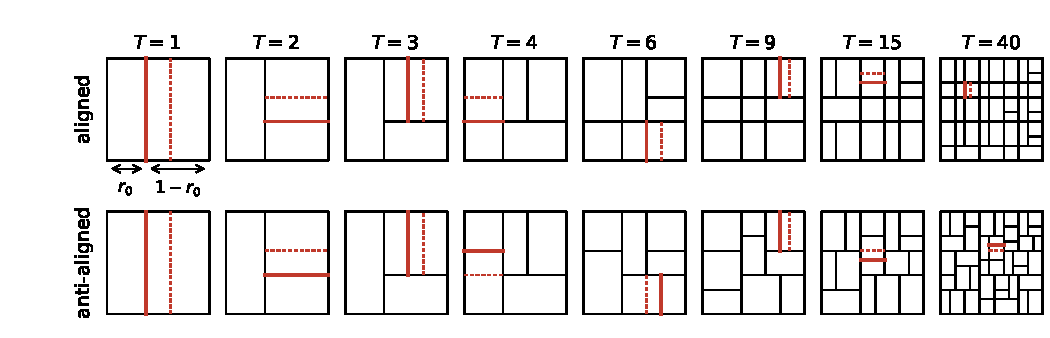
\includegraphics[width=\textwidth]{figS1.pdf}
\caption{Recursive cell division with the golden split $r_0=\tau^{-2}$, after $T$ cuts. At each
step the largest cell is cut perpendicular to its long side, at a fraction $r_0$ of its length
measured from one of its two ends. Red: the newest cut; dashed: the other candidate position.
Top, aligned rule: $r_0$ is always measured from the low end (left or bottom). Bottom,
anti-aligned rule: $r_0$ is measured from the end whose cut forms fewer X-crossings. The two
rows agree up to $T=3$; at $T=4$ the aligned cut would continue the cut of $T=2$ across the
first cut, and the anti-aligned rule takes the other position.}
\label{fig:steps}
\end{figure}

Figure~\ref{fig:steps} shows the first steps of the division of the unit square. Each cut is a
ligament that ends on two existing ligaments, its hosts, and forms a T-junction with each. Under
the aligned rule the cuts of neighbouring cells line up and join into straight lines that span
the square. Under the anti-aligned rule a cut moves to the other candidate position whenever
that avoids continuing a cut on the other side of a host.

\begin{figure}[h]
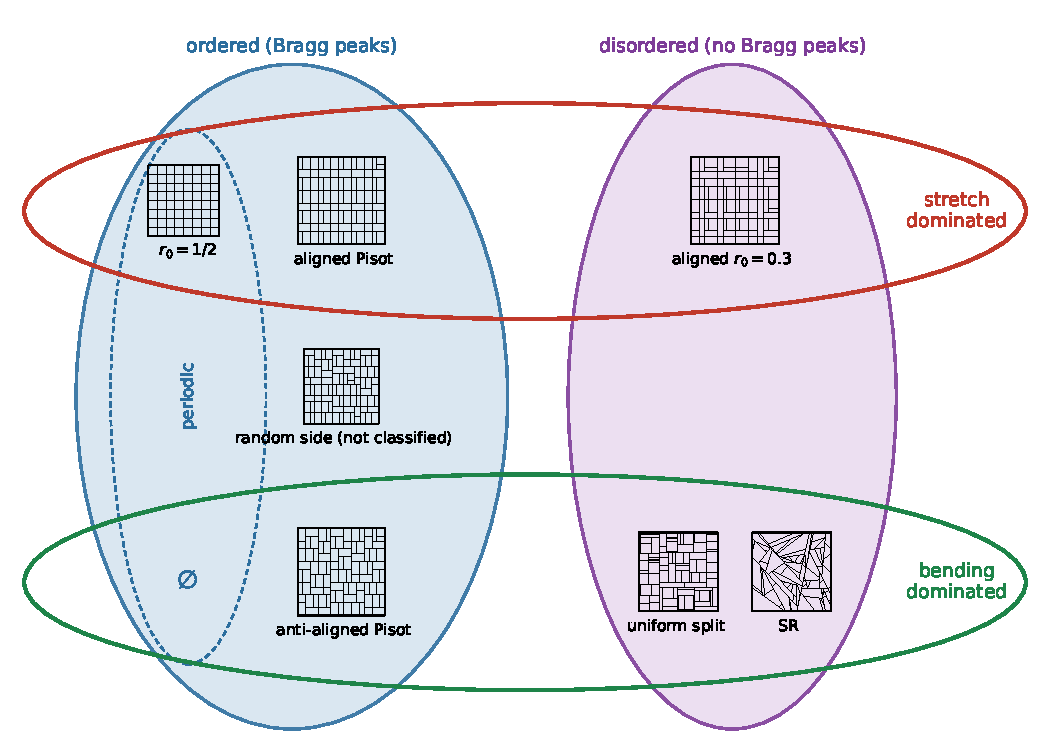
\includegraphics[width=0.85\textwidth]{figS2.pdf}
\caption{Order and alignment classes of the divisions. Each oval is one property: ordered (Bragg
peaks) or disordered (no Bragg peaks), and aligned or non-aligned (number of spanning lines
$m\propto T^{\mu}$ with $\mu=1/2$ or $\mu=0$). Ordered and disordered exclude each other, as do
aligned and non-aligned, so the four overlaps are the four classes. All four are realised. The
alignment class sets the elasticity (in brackets): aligned frameworks are stretch dominated,
non-aligned ones bending dominated. The periodic grid ($r_0=1/2$, dashed sub-oval) has no
anti-aligned version, so periodic and non-aligned is empty. The random-side golden split is
ordered and partially aligned, $\mu\approx0.2$, between the two ovals; its stretching share was
not computed. Thumbnails after $T=89$ cuts ($T=63$ for $r_0=1/2$). Members of one overlap share a
class, not the values of their elastic constants.}
\label{fig:classes}
\end{figure}

Figure~\ref{fig:classes} places the divisions in the classes defined by the two properties.
The value of $r_0$ moves a division between the ordered and disordered ovals; the side rule
moves it between the aligned and non-aligned ovals. The anti-aligned Pisot splits share the
non-aligned class, and with it bending domination, with the random uniform split and the
scale-rich rule, but not the order class. Within that class they are less compliant: at $T=10^{3}$ and $\bar\rho=0.1$ their
rigid-joint index is $78$--$94\%$ of the scale-rich value, and the ratio falls with density.

\section{Scaling of the number of spanning lines}

Let $r_{\min}=\min(r_0,1-r_0)$ and let $m=m_h+m_v$ count the straight lines that span the unit
square, the frame excluded. We show that $m\propto T^{1/2}$ for the aligned rule and $m\lesssim
T^{1/2}$ for every side rule.

\textit{Lemma 1 (area window).} After $T$ cuts the $T+1$ cells have areas in $[r_{\min}A_{\max},
A_{\max}]$, with $A_{\max}$ the current largest area. Indeed, each cell was created by cutting
the largest cell of that moment, whose area is at least the current $A_{\max}$ because areas only
decrease, and it received at least the fraction $r_{\min}$ of it. Since the areas add up to one,
$1/(T+1)\le A_{\max}\le 1/[r_{\min}(T+1)]$.

\textit{Lemma 2 (aspect ratio).} Every cell has aspect ratio $\alpha$ (long side over short side)
at most $1/r_{\min}$. The square has $\alpha=1$. Cut a cell with sides $L\ge S$ and
$\alpha=L/S\le1/r_{\min}$ perpendicular to $L$; a daughter has sides $rL$ and $S$ with $r\ge
r_{\min}$. If $rL\ge S$ its aspect ratio is $rL/S\le\alpha$; otherwise it is $S/(rL)=1/(r\alpha)\le
1/r_{\min}$, because $\alpha\ge1$. The bound is attained (numerically, $2.618$ for the golden
split).

Together, every side $w$ of every cell satisfies
\begin{equation}
\frac{r_{\min}}{\sqrt{T+1}}\le w\le\frac{1}{r_{\min}\sqrt{T+1}} ,
\label{eq:wbounds}
\end{equation}
since $w^{2}$ lies between $A_{\min}/\alpha_{\max}\ge r_{\min}^{2}/(T+1)$ and
$A_{\max}\alpha_{\max}\le1/[r_{\min}^{2}(T+1)]$.

\textit{Upper bound, any side rule.} A vertical spanning line meets the bottom edge of the
square at a junction between two cells that touch that edge. These cells have widths at least
$w_{\min}$, so there are at most $1/w_{\min}$ of them and $m_v\le1/w_{\min}-1$. With the same
argument for $m_h$,
\begin{equation}
m\le2\left(\frac{\sqrt{T+1}}{r_{\min}}-1\right).
\label{eq:mup}
\end{equation}
Hence $\mu\le1/2$ for every side rule with fixed $r_0$.

\textit{Lower bound, aligned rule.} In the aligned rule the division is a partially refined
product of two one-dimensional $r_0$-splittings $X$ and $Y$ (Letter): every cell is $I\times J$
with $I$ a node of the splitting tree of $X$ and $J$ one of $Y$. Take a node $I$ of $X$ longer
than the largest current width $w_{\max}$. A cell of $x$-extent $I$ is removed either by a horizontal cut, which leaves two cells of
$x$-extent $I$, or by a vertical cut, always at the same point $x_0+r_0|I|$. The cells of
$x$-extent $I$ tile the strip $I\times[0,1]$, because the $x$-extents form a tree. No current
cell has $x$-extent $I$, so the whole strip has been cut at $x_0+r_0|I|$, and these vertical
cuts join into a line that spans the square. The nodes of $X$ longer than $w_{\max}$ form a subtree; its children that are not in it
partition $[0,1]$ into intervals of length at most $w_{\max}$, so there are at least
$1/w_{\max}$ of them and at least $1/w_{\max}-1$ split points. With Eq.~(\ref{eq:wbounds}) and
the same argument for $Y$,
\begin{equation}
m\ge2\left(r_{\min}\sqrt{T+1}-1\right).
\label{eq:mlow}
\end{equation}
Equations~(\ref{eq:mup}) and (\ref{eq:mlow}) give $m=a(T)\,T^{1/2}$ with
$2r_{\min}\le a\le2/r_{\min}$ asymptotically, so $\mu=1/2$ exactly for the aligned rule. For the
golden split the bounds are $0.76$ and $5.2$; the measured $a=m/\sqrt{T+1}$ lies between $1.45$
and $1.71$ for $T=10^{3}$--$10^{6}$, and $1.35$--$1.43$ for $r_0=0.3$. The prefactor varies
non-monotonically with $T$ within the bounds, as expected from largest-first division, which
refines the cells in generations whose areas repeat on a geometric scale.

\textit{Other side rules.} Equation~(\ref{eq:mup}) bounds $\mu\le1/2$, but the lower bound uses
the product structure and does not extend. For the anti-aligned rule $m=1$, so $\mu=0$, is
observed, not derived (next section). For the random side the fitted $\mu=0.21\pm0.01$ lies between
the two bounds; we have no derivation of its value.

\section{Anti-aligned rule}\label{sec:anti}

The cell to be cut is the largest one; the cut is perpendicular to its long side. The two
candidate positions are $r_0$ and $1-r_0$ of the extent across the cut. A candidate forms a
crossing at an end if a junction of a stem from the other side of the host ligament lies at
exactly that position on the host. For each candidate the crossings at its two ends are
counted (0, 1 or 2); the candidate with fewer crossings is taken, and a tie goes to $r_0$ on
the low side (left or bottom). The first cut of the square meets the frame only, so it lies
at $x=r_0$. The rule is deterministic.

With this rule the axis Bragg weight of the golden junction set fluctuates between $0.53$ and
$0.62$ for $T=4095$--$1048575$, that of $(5,1)$ between $0.11$ and $0.14$, and that of $(3,2)$
between $0.08$ and $0.11$. Only the first cut spans the square ($m=1$) for all five Pisot
splits up to $T=10^{6}$. The longest straight line other than the first cut has length
$1-r_0$ for all three anti-aligned splits (column longest$_2$ of Table~\ref{tab:geo}) at
every $T$: it is the second cut, and no later line grows beyond it.

\section{Beam model}

\textit{Network.} Each ligament is divided into segments at the junctions it hosts.
Coincident junctions (X-crossings) are merged into a single rigid joint. The frame of the
square is a ligament of the same thickness as the others.

\textit{Tiling.} The division and its three mirror images form a $2\times2$ supercell, which
is tiled periodically; the frame is shared between neighbouring tiles and counted once.

\textit{Elements.} Euler--Bernoulli frame elements with $E=1$ and unit depth: axial stiffness
$EA=E\lambda$, bending stiffness $EI=E\lambda^{3}/12$. All ligaments have the same thickness
$\lambda=\bar\rho/L_{\rm tot}$. A segment shorter than its thickness lies inside a junction
block; its stiffness length is $\max(\ell,\lambda)$. Pinned joints: $EI=0$.

\textit{Effective stiffness.} For each macroscopic strain $\varepsilon\in\{\varepsilon_{xx},
\varepsilon_{yy},\gamma_{xy}\}$ the displacement is the affine field plus a periodic
fluctuation that minimises the energy, $U=U_{\rm aff}+Pw$, with $P$ the periodic map. Then
$C=U^{\rm T}KU/A$ with $A=4$ the supercell area.

\textit{Index.} With the solid density $\rho_s=1$ and $c_0=\sqrt{E/\rho_s}=1$, the
longitudinal index along direction $\phi$ is $n(\phi)=\sqrt{\bar\rho/\Lambda_{\max}(\phi)}$,
with $\Lambda_{\max}$ the largest eigenvalue of the Christoffel matrix of $C$;
$\langle n\rangle$ averages $n(\phi)$ over 72 directions in $[0,\pi)$.

\textit{Exact pinned stiffness.} Equation~(2) of the Letter agrees with the finite-element
$C^{\rm pin}$ to machine precision for aligned, random-side and anti-aligned divisions.

\section{Stretching share}

Rigid joints add the positive semidefinite bending matrix $K^{\rm b}$ to the axial matrix
$K^{\rm a}$, so $C\ge C^{\rm pin}$. The Letter uses
\begin{equation}
s=\frac{\mathrm{tr}\,C^{\rm pin}}{\mathrm{tr}\,C},
\end{equation}
the fraction of the stiffness that survives when the joints are pinned. This is the
criterion of Deshpande, Ashby and Fleck: a framework is bending dominated when it loses its
stiffness on pinning the joints. A second measure is the axial share of the rigid-joint strain
energy, $s_E=\mathrm{tr}(U^{\rm T}K^{\rm a}U)/\mathrm{tr}(U^{\rm T}KU)$. Because the rigid-joint
displacement does not minimise the axial energy alone, $s_E\ge s$.

Table~\ref{tab:T4} gives both at $T=10^{4}$. In the aligned split both are close to one. In
the anti-aligned splits and the uniform split, $s$ is small and falls with $T$
(Table~\ref{tab:size}), while $s_E$ stays between $0.3$ and $0.5$: the members of a
rigid-jointed rectangular framework stretch as well as bend when a T-junction host deflects.
The decrease of $s$ with $T$ at fixed $\bar\rho$ is the size dependence predicted by Eq.~(4)
of the Letter. Fits over $T=300$--$10^{4}$ give $s/(1-s)\propto T^{-\beta}$ with
$\beta=0.50$--$0.53$ (golden and $(3,2)$ anti-aligned), $0.57$--$0.63$ ($(5,1)$ anti-aligned)
and $0.37$--$0.44$ (uniform split), for $\bar\rho=0.05$--$0.2$. The density dependence is
weaker than the $\bar\rho^{-2}$ of Eq.~(4): at $T=10^{4}$, $s/(1-s)\propto\bar\rho^{-1.56}$ to
$\bar\rho^{-1.60}$ for the three anti-aligned splits and the uniform split. The departure is
probably the axial contribution measured by $s_E$, which makes $C-C^{\rm pin}$ grow more slowly
than $\bar\rho^{3}$. The collapse of Fig.~3(c) of the Letter is therefore approximate in
$\bar\rho$ and holds in $T$.

The rigid-joint index grows much more slowly than the pinned ceiling, which grows as
$T^{1/4}$ (Table~\ref{tab:size}): fits give $\langle n\rangle\propto T^{0.06-0.07}$ for the
anti-aligned splits and $T^{0.13}$ for the uniform split at $\bar\rho=0.1$. Both are consistent
with Eq.~(4), since $C\to C^{\rm b}$, independent of $T$, as $s\to0$.

For aligned divisions $m+1\propto L_{\rm tot}$ and $s$ stays above $0.9$ at every size, but
$s/(1-s)$ does not follow $\bar\rho^{-2}$ (exponent $-0.47$ at $T=10^{4}$) and is not monotonic
in $T$. The incomplete parts of the grid lines, which hold $5$--$33\%$ of the ligament length,
carry axial load through the rigid joints, so $C-C^{\rm pin}$ is not a pure bending term. The
Letter applies Eq.~(4) only to $m=1$.

\section{Slenderness and Timoshenko beams}

Lengths are given in units of $1/L_{\rm tot}$, in which a length $\ell$ equals $\ell
L_{\rm tot}/\bar\rho$ thicknesses (Table~\ref{tab:geo}). For $\bar\rho\le0.1$ at most $2.4\%$
of the segments of any anti-aligned split are shorter than $3\lambda$; at $\bar\rho=0.2$ this
remains true only for the golden split. Replacing Euler--Bernoulli by Timoshenko elements, with
shear parameter $\Phi=12EI/(\kappa GA\ell^{2})$, $G=E/[2(1+\nu)]$, changes $\langle n\rangle$
by a few percent (Table~\ref{tab:timo}).

\section{Offsets and the finite-thickness test}

Two stems on opposite sides of a host at distance $\delta$ form a jogged line. For a Meyer set
the difference set is uniformly discrete, so $\delta$ is bounded below in units of the
smallest cell. The bound is approached slowly for the plastic splits, whose minimum offset
still decreases at $T=10^{5}$; the first percentile is stable (Table~\ref{tab:geo}).

The finite-thickness test treats parallel ligaments whose centre lines are closer than
$\lambda$ as one: coordinates within $\lambda$ are merged by single linkage and the spanning
lines are recounted. Table~\ref{tab:snap} gives the largest density at which $m=1$ survives.
Above it spanning lines reappear in numbers that grow with $T$, and the anti-aligned division
crosses over to the aligned class. Offsets and thickness both scale as $T^{-1/2}$, so the
threshold does not drift with $T$ for the golden split. For $(5,1)$ it drifts slowly, from
$0.30$ to $0.25$ between $T=10^{3}$ and $10^{6}$, following the slow decrease of $\delta_{\min}$;
the range $\bar\rho\lesssim0.1$ stated for the plastic splits leaves a margin.

\section{Beyond elasticity: properties set by both classes}

The two labels of a division have distinct geometric origins. The order class comes from the
arithmetic of $r_0$: it fixes where the junctions lie and therefore the Bragg peaks. The
alignment class comes from the side rule: it fixes which cuts continue each other across a host
(X-crossings) and how many straight lines span the sample. A property that probes only one of
these features follows only one label. Diffraction sees only the order. The long-wavelength
stiffness sees only the alignment (Letter). Scalar transport, such as electrical
conduction through the ligaments, depends on connectivity alone and follows neither, as the
dual graph does not. Waves that travel inside the network at wavelengths comparable to the cell
size are different: the order sets which frequencies propagate, and the side rule sets along
which paths. The four properties below should therefore depend on both labels. None has been
computed here; they are predictions. The aligned and anti-aligned golden splits are the
controlled pair for testing them: both are Meyer sets with Bragg peaks and three cell shapes,
and they differ only in their straight lines.

\textit{Elastic waves at finite frequency.} The Letter treats the limit of long wavelength,
where the index is set by the stiffness. At wavelengths of the order of the cell size, Bragg
scattering opens band gaps. Their positions are drawn from the Bragg peaks of the junction
set, which lie in the same Fourier module for both side rules; their widths follow the peak
intensities, which differ (Fig.~2 of the Letter). Inside the bands the side rule takes over.
In an aligned division a longitudinal wave can run along a spanning line, a continuous beam
loaded at its junctions, as in a one-dimensional quasiperiodic chain. In an anti-aligned
division every straight path ends at a T-junction on a perpendicular beam, where the
longitudinal wave is converted into flexural motion. The prediction is gaps at related
frequencies in both, with guided propagation within the bands for the aligned division and
scattered, possibly localised, propagation for the anti-aligned one. The Bloch-wave
calculation on the framed periodic tiling used for scale-rich metamaterials
(\texttt{beyond/blochsweep.py}) gives the dispersion and the plane-wave content of each mode and
can test this directly.

\textit{Electrons on networks of quantum wires.} Consider electrons hopping between junctions
along the ligaments (a tight-binding model on the junction network), or waves on the ligaments
with current conservation at each junction (a quantum graph). The order class sets the
character of the spectrum: one-dimensional quasiperiodic chains such as the Fibonacci chain
have Cantor-set spectra and critical states. The side rule sets whether the problem separates.
The complete aligned division is a product grid, so its Hamiltonian is
$H=H_X\otimes1+1\otimes H_Y$, with $H_X$ and $H_Y$ the chains of the two one-dimensional
splittings. Its spectrum is the sum of two one-dimensional spectra, as for the square Fibonacci
tiling~\cite{evendar2006,evendar2008}. The incomplete grid lines, which hold $5$--$33\%$ of the
ligament length, break this separation weakly. The anti-aligned division has the same order
class but no product structure, and its Hamiltonian does not separate. Comparing the two
isolates the effect of separability at fixed quasiperiodic order on the spectrum and on the
localisation of states. A magnetic field adds an Aharonov--Bohm phase proportional to the flux
through each cell. For Pisot splits the cell areas take finitely many values, three for the
golden split, so the phases are themselves quasiperiodic. In superconducting wire networks
the field dependence of the transition temperature follows this spectrum, as measured on
Penrose networks~\cite{behrooz1986}. It would carry both labels, the area spectrum through the
order and the loop structure through the side rule.

\textit{Spin waves in magnetic wire networks.} In connected ferromagnetic nanowires the
magnetisation lies along each wire. Spin waves propagate along the wires and scatter at
junctions, and magnetisation reversal proceeds by domain walls that move along the wires and
are pinned at junctions. At an X-crossing a wire continues straight through. At a T-junction
it ends on a perpendicular wire, where the magnetisation must turn, which scatters spin waves
and pins domain walls. The magnon bands should inherit the quasiperiodic gaps of the order
class. The side rule should set the propagation: spanning lines in aligned networks provide
channels for spin waves and paths for reversal across the whole sample, while in anti-aligned
networks most straight segments are of the order of the cell size, which confines spin waves
and breaks reversal into avalanches bounded by the lengths of the straight lines.

\textit{Phonon heat conduction.} Heat in the framework is carried by its elastic waves, so the
thermal conductivity combines the two previous effects, weighted by the thermal population of
the modes. At the lowest temperatures only long-wavelength modes are populated, the
conductivity follows the sound speed, and only the side rule matters, through the index $n$.
At temperatures where the dominant phonon wavelength is comparable to the cell size, the gaps
of the order class remove modes, and the straight lines of the side rule decide whether the
remaining modes travel ballistically, along spanning lines, or diffusively. The temperature
dependence of the conductivity should therefore cross over from a single-label to a two-label
regime.

\begin{table}[h]\caption{Rigid-joint beam model at $T=10^{4}$ (uniform split: one realisation; over three realisations at $T=3000$ the relative spread is below $2\%$ in $\langle n\rangle$ and $3\%$ in $s$). $\langle n\rangle$: direction-averaged index; $s=\mathrm{tr}\,C^{\rm pin}/\mathrm{tr}\,C$; $s_E$: axial part of the rigid-joint strain energy.}\label{tab:T4}
\begin{ruledtabular}\begin{tabular}{lccccccccc}
 & \multicolumn{3}{c}{$\bar\rho=0.05$} & \multicolumn{3}{c}{$\bar\rho=0.1$} & \multicolumn{3}{c}{$\bar\rho=0.2$} \\
rule & $\langle n\rangle$ & $s$ & $s_E$ & $\langle n\rangle$ & $s$ & $s_E$ & $\langle n\rangle$ & $s$ & $s_E$ \\ \hline
golden, aligned & 1.84 & 0.953 & 0.99 & 1.82 & 0.936 & 0.99 & 1.80 & 0.914 & 0.98 \\
golden, anti & 8.01 & 0.352 & 0.41 & 5.09 & 0.143 & 0.32 & 3.24 & 0.058 & 0.41 \\
(5,1), anti & 8.61 & 0.401 & 0.46 & 5.59 & 0.170 & 0.34 & 3.59 & 0.071 & 0.42 \\
(3,2), anti & 7.52 & 0.323 & 0.38 & 4.66 & 0.125 & 0.29 & 2.92 & 0.050 & 0.41 \\
uniform split & 10.18 & 0.541 & 0.60 & 7.12 & 0.267 & 0.41 & 4.71 & 0.117 & 0.41 \\
\end{tabular}\end{ruledtabular}\end{table}
\begin{table}[h]\caption{Size dependence at $\bar\rho=0.1$: rigid-joint $\langle n\rangle$, pinned ceiling $n_{\max,x}$ and stretching share $s$ (uniform split: mean of three realisations for $T<10^4$).}\label{tab:size}
\begin{ruledtabular}\begin{tabular}{lcccccccc}
rule & \multicolumn{2}{c}{$T=300$} & \multicolumn{2}{c}{$T=1000$} & \multicolumn{2}{c}{$T=3000$} & \multicolumn{2}{c}{$T=10000$} \\
 & $\langle n\rangle$, $n_{\max,x}$ & $s$ & $\langle n\rangle$, $n_{\max,x}$ & $s$ & $\langle n\rangle$, $n_{\max,x}$ & $s$ & $\langle n\rangle$, $n_{\max,x}$ & $s$ \\ \hline
golden, aligned & 1.78, 1.65 & 0.952 & 1.74, 1.76 & 0.997 & 1.78, 1.79 & 0.993 & 1.82, 1.87 & 0.936 \\
golden, anti & 3.96, 5.96 & 0.497 & 4.55, 8.05 & 0.358 & 4.85, 10.59 & 0.235 & 5.09, 14.37 & 0.143 \\
(5,1), anti & 4.46, 6.10 & 0.621 & 4.99, 8.24 & 0.426 & 5.15, 10.86 & 0.262 & 5.59, 14.65 & 0.170 \\
(3,2), anti & 3.75, 5.93 & 0.465 & 4.15, 8.02 & 0.311 & 4.49, 10.56 & 0.212 & 4.66, 14.28 & 0.125 \\
uniform split & 4.49, 6.28 & 0.605 & 5.59, 8.47 & 0.517 & 6.52, 11.14 & 0.407 & 7.12, 15.04 & 0.267 \\
\end{tabular}\end{ruledtabular}\end{table}
\begin{table}[h]\caption{Relative change of $\langle n\rangle$ from Euler--Bernoulli to Timoshenko beams ($\nu=0.3$, $\kappa=5/6$), maximum over $T=300$--$10^{4}$.}\label{tab:timo}
\begin{ruledtabular}\begin{tabular}{lcc}rule & $\bar\rho=0.2$ & $\bar\rho=0.4$ \\ \hline
golden, aligned & 0.1\% & 0.4\% \\
golden, anti & 2.1\% & 5.5\% \\
(5,1), anti & 2.3\% & 5.6\% \\
(3,2), anti & 3.1\% & 7.1\% \\
uniform split & 1.9\% & 4.7\% \\
\end{tabular}\end{ruledtabular}\end{table}
\begin{table}[h]\caption{Geometry in units of $1/L_{\rm tot}$, so that a length $\ell$ equals $\ell L_{\rm tot}/\bar\rho$ thicknesses. Segments between consecutive joints: minimum and median; fraction shorter than $3\lambda$ at $\bar\rho=0.1$ and $0.2$. Offsets $\delta$ between opposite stems on a host: minimum and first percentile.}\label{tab:geo}
\begin{ruledtabular}\begin{tabular}{lcccccccc}
rule & $T$ & $\ell_{\min}$ & $\ell_{\rm med}$ & $f_{<3\lambda}(0.1)$ & $f_{<3\lambda}(0.2)$ & $\delta_{\min}$ & $\delta_{1\%}$ & longest$_2$ \\ \hline
golden, anti & $10^{3}$ & 0.32 & 1.34 & 0.000 & 0.019 & 0.32 & 0.51 & 0.618 \\
golden, anti & $10^{4}$ & 0.39 & 1.66 & 0.000 & 0.005 & 0.39 & 0.39 & 0.618 \\
golden, anti & $10^{5}$ & 0.47 & 1.24 & 0.000 & 0.013 & 0.47 & 0.47 & 0.618 \\
(5,1), anti & $10^{3}$ & 0.14 & 1.29 & 0.021 & 0.146 & 0.14 & 0.18 & 0.755 \\
(5,1), anti & $10^{4}$ & 0.11 & 1.35 & 0.021 & 0.157 & 0.11 & 0.19 & 0.755 \\
(5,1), anti & $10^{5}$ & 0.08 & 1.39 & 0.024 & 0.160 & 0.08 & 0.19 & 0.755 \\
(3,2), anti & $10^{3}$ & 0.30 & 1.22 & 0.001 & 0.158 & 0.30 & 0.40 & 0.570 \\
(3,2), anti & $10^{4}$ & 0.24 & 1.28 & 0.000 & 0.168 & 0.24 & 0.42 & 0.570 \\
(3,2), anti & $10^{5}$ & 0.18 & 1.32 & 0.000 & 0.177 & 0.18 & 0.32 & 0.570 \\
golden, aligned & $10^{3}$ & 0.83 & 2.16 & 0.000 & 0.000 & 0.83 & 0.89 & 1.000 \\
golden, aligned & $10^{4}$ & 1.03 & 1.67 & 0.000 & 0.000 & 1.03 & 1.03 & 1.000 \\
golden, aligned & $10^{5}$ & 1.24 & 2.01 & 0.000 & 0.000 & 1.24 & 1.24 & 1.000 \\
\end{tabular}\end{ruledtabular}\end{table}
\begin{table}[h]\caption{Finite-thickness test: largest $\bar\rho$ (step $0.05$) at which merging parallel ligaments closer than $\lambda$ leaves $m=1$.}\label{tab:snap}
\begin{ruledtabular}\begin{tabular}{lcccc}rule & $T=10^{3}$ & $10^{4}$ & $10^{5}$ & $10^{6}$ \\ \hline
golden, anti & 0.50 & 0.60 & 0.75 & 0.55 \\
(5,1), anti & 0.30 & 0.30 & 0.25 & 0.25 \\
(3,2), anti & 0.35 & 0.40 & 0.30 & 0.30 \\
\end{tabular}\end{ruledtabular}\end{table}


\bibliography{refs}

\end{document}
